\documentclass[]{article}
\usepackage{lmodern}
\usepackage{amssymb,amsmath}
\usepackage{ifxetex,ifluatex}
\usepackage{fixltx2e} % provides \textsubscript
\ifnum 0\ifxetex 1\fi\ifluatex 1\fi=0 % if pdftex
  \usepackage[T1]{fontenc}
  \usepackage[utf8]{inputenc}
\else % if luatex or xelatex
  \ifxetex
    \usepackage{mathspec}
  \else
    \usepackage{fontspec}
  \fi
  \defaultfontfeatures{Ligatures=TeX,Scale=MatchLowercase}
\fi
% use upquote if available, for straight quotes in verbatim environments
\IfFileExists{upquote.sty}{\usepackage{upquote}}{}
% use microtype if available
\IfFileExists{microtype.sty}{%
\usepackage{microtype}
\UseMicrotypeSet[protrusion]{basicmath} % disable protrusion for tt fonts
}{}
\usepackage[margin=1in]{geometry}
\usepackage{hyperref}
\hypersetup{unicode=true,
            pdftitle={heatmap\_final},
            pdfauthor={GG},
            pdfborder={0 0 0},
            breaklinks=true}
\urlstyle{same}  % don't use monospace font for urls
\usepackage{color}
\usepackage{fancyvrb}
\newcommand{\VerbBar}{|}
\newcommand{\VERB}{\Verb[commandchars=\\\{\}]}
\DefineVerbatimEnvironment{Highlighting}{Verbatim}{commandchars=\\\{\}}
% Add ',fontsize=\small' for more characters per line
\usepackage{framed}
\definecolor{shadecolor}{RGB}{248,248,248}
\newenvironment{Shaded}{\begin{snugshade}}{\end{snugshade}}
\newcommand{\KeywordTok}[1]{\textcolor[rgb]{0.13,0.29,0.53}{\textbf{#1}}}
\newcommand{\DataTypeTok}[1]{\textcolor[rgb]{0.13,0.29,0.53}{#1}}
\newcommand{\DecValTok}[1]{\textcolor[rgb]{0.00,0.00,0.81}{#1}}
\newcommand{\BaseNTok}[1]{\textcolor[rgb]{0.00,0.00,0.81}{#1}}
\newcommand{\FloatTok}[1]{\textcolor[rgb]{0.00,0.00,0.81}{#1}}
\newcommand{\ConstantTok}[1]{\textcolor[rgb]{0.00,0.00,0.00}{#1}}
\newcommand{\CharTok}[1]{\textcolor[rgb]{0.31,0.60,0.02}{#1}}
\newcommand{\SpecialCharTok}[1]{\textcolor[rgb]{0.00,0.00,0.00}{#1}}
\newcommand{\StringTok}[1]{\textcolor[rgb]{0.31,0.60,0.02}{#1}}
\newcommand{\VerbatimStringTok}[1]{\textcolor[rgb]{0.31,0.60,0.02}{#1}}
\newcommand{\SpecialStringTok}[1]{\textcolor[rgb]{0.31,0.60,0.02}{#1}}
\newcommand{\ImportTok}[1]{#1}
\newcommand{\CommentTok}[1]{\textcolor[rgb]{0.56,0.35,0.01}{\textit{#1}}}
\newcommand{\DocumentationTok}[1]{\textcolor[rgb]{0.56,0.35,0.01}{\textbf{\textit{#1}}}}
\newcommand{\AnnotationTok}[1]{\textcolor[rgb]{0.56,0.35,0.01}{\textbf{\textit{#1}}}}
\newcommand{\CommentVarTok}[1]{\textcolor[rgb]{0.56,0.35,0.01}{\textbf{\textit{#1}}}}
\newcommand{\OtherTok}[1]{\textcolor[rgb]{0.56,0.35,0.01}{#1}}
\newcommand{\FunctionTok}[1]{\textcolor[rgb]{0.00,0.00,0.00}{#1}}
\newcommand{\VariableTok}[1]{\textcolor[rgb]{0.00,0.00,0.00}{#1}}
\newcommand{\ControlFlowTok}[1]{\textcolor[rgb]{0.13,0.29,0.53}{\textbf{#1}}}
\newcommand{\OperatorTok}[1]{\textcolor[rgb]{0.81,0.36,0.00}{\textbf{#1}}}
\newcommand{\BuiltInTok}[1]{#1}
\newcommand{\ExtensionTok}[1]{#1}
\newcommand{\PreprocessorTok}[1]{\textcolor[rgb]{0.56,0.35,0.01}{\textit{#1}}}
\newcommand{\AttributeTok}[1]{\textcolor[rgb]{0.77,0.63,0.00}{#1}}
\newcommand{\RegionMarkerTok}[1]{#1}
\newcommand{\InformationTok}[1]{\textcolor[rgb]{0.56,0.35,0.01}{\textbf{\textit{#1}}}}
\newcommand{\WarningTok}[1]{\textcolor[rgb]{0.56,0.35,0.01}{\textbf{\textit{#1}}}}
\newcommand{\AlertTok}[1]{\textcolor[rgb]{0.94,0.16,0.16}{#1}}
\newcommand{\ErrorTok}[1]{\textcolor[rgb]{0.64,0.00,0.00}{\textbf{#1}}}
\newcommand{\NormalTok}[1]{#1}
\usepackage{graphicx,grffile}
\makeatletter
\def\maxwidth{\ifdim\Gin@nat@width>\linewidth\linewidth\else\Gin@nat@width\fi}
\def\maxheight{\ifdim\Gin@nat@height>\textheight\textheight\else\Gin@nat@height\fi}
\makeatother
% Scale images if necessary, so that they will not overflow the page
% margins by default, and it is still possible to overwrite the defaults
% using explicit options in \includegraphics[width, height, ...]{}
\setkeys{Gin}{width=\maxwidth,height=\maxheight,keepaspectratio}
\IfFileExists{parskip.sty}{%
\usepackage{parskip}
}{% else
\setlength{\parindent}{0pt}
\setlength{\parskip}{6pt plus 2pt minus 1pt}
}
\setlength{\emergencystretch}{3em}  % prevent overfull lines
\providecommand{\tightlist}{%
  \setlength{\itemsep}{0pt}\setlength{\parskip}{0pt}}
\setcounter{secnumdepth}{0}
% Redefines (sub)paragraphs to behave more like sections
\ifx\paragraph\undefined\else
\let\oldparagraph\paragraph
\renewcommand{\paragraph}[1]{\oldparagraph{#1}\mbox{}}
\fi
\ifx\subparagraph\undefined\else
\let\oldsubparagraph\subparagraph
\renewcommand{\subparagraph}[1]{\oldsubparagraph{#1}\mbox{}}
\fi

%%% Use protect on footnotes to avoid problems with footnotes in titles
\let\rmarkdownfootnote\footnote%
\def\footnote{\protect\rmarkdownfootnote}

%%% Change title format to be more compact
\usepackage{titling}

% Create subtitle command for use in maketitle
\newcommand{\subtitle}[1]{
  \posttitle{
    \begin{center}\large#1\end{center}
    }
}

\setlength{\droptitle}{-2em}
  \title{heatmap\_final}
  \pretitle{\vspace{\droptitle}\centering\huge}
  \posttitle{\par}
  \author{GG}
  \preauthor{\centering\large\emph}
  \postauthor{\par}
  \predate{\centering\large\emph}
  \postdate{\par}
  \date{1/28/2019}


\begin{document}
\maketitle

Loading Libraries

\begin{Shaded}
\begin{Highlighting}[]
\KeywordTok{library}\NormalTok{(ggplot2)}
\KeywordTok{library}\NormalTok{(tidyverse)}
\end{Highlighting}
\end{Shaded}

\begin{verbatim}
## -- Attaching packages --------------------------------------- tidyverse 1.2.1 --
\end{verbatim}

\begin{verbatim}
## √ tibble  1.4.2     √ purrr   0.2.4
## √ tidyr   0.8.0     √ dplyr   0.7.4
## √ readr   1.1.1     √ stringr 1.3.0
## √ tibble  1.4.2     √ forcats 0.3.0
\end{verbatim}

\begin{verbatim}
## -- Conflicts ------------------------------------------ tidyverse_conflicts() --
## x dplyr::filter() masks stats::filter()
## x dplyr::lag()    masks stats::lag()
\end{verbatim}

\begin{Shaded}
\begin{Highlighting}[]
\KeywordTok{library}\NormalTok{(readxl)}
\KeywordTok{library}\NormalTok{(janitor)}
\KeywordTok{library}\NormalTok{(dbplyr)}
\end{Highlighting}
\end{Shaded}

\begin{verbatim}
## 
## Attaching package: 'dbplyr'
\end{verbatim}

\begin{verbatim}
## The following objects are masked from 'package:dplyr':
## 
##     ident, sql
\end{verbatim}

Input datafile from computer

\begin{Shaded}
\begin{Highlighting}[]
\NormalTok{heatmap <-}\StringTok{ }\KeywordTok{read_csv}\NormalTok{(}\StringTok{"~/Desktop/Lionfish/Heatmap data.csv"}\NormalTok{)}
\end{Highlighting}
\end{Shaded}

\begin{verbatim}
## Parsed with column specification:
## cols(
##   species = col_character(),
##   site = col_character(),
##   sum = col_double(),
##   mean = col_double()
## )
\end{verbatim}

plot data Basic Heatplot

\begin{Shaded}
\begin{Highlighting}[]
\KeywordTok{ggplot}\NormalTok{(}\DataTypeTok{data =}\NormalTok{ heatmap, }\KeywordTok{aes}\NormalTok{(}\DataTypeTok{x =}\NormalTok{ site, }\DataTypeTok{y =}\NormalTok{ species)) }\OperatorTok{+}\StringTok{ }\KeywordTok{geom_tile}\NormalTok{(}\KeywordTok{aes}\NormalTok{(}\DataTypeTok{fill =}\NormalTok{ mean))}
\end{Highlighting}
\end{Shaded}

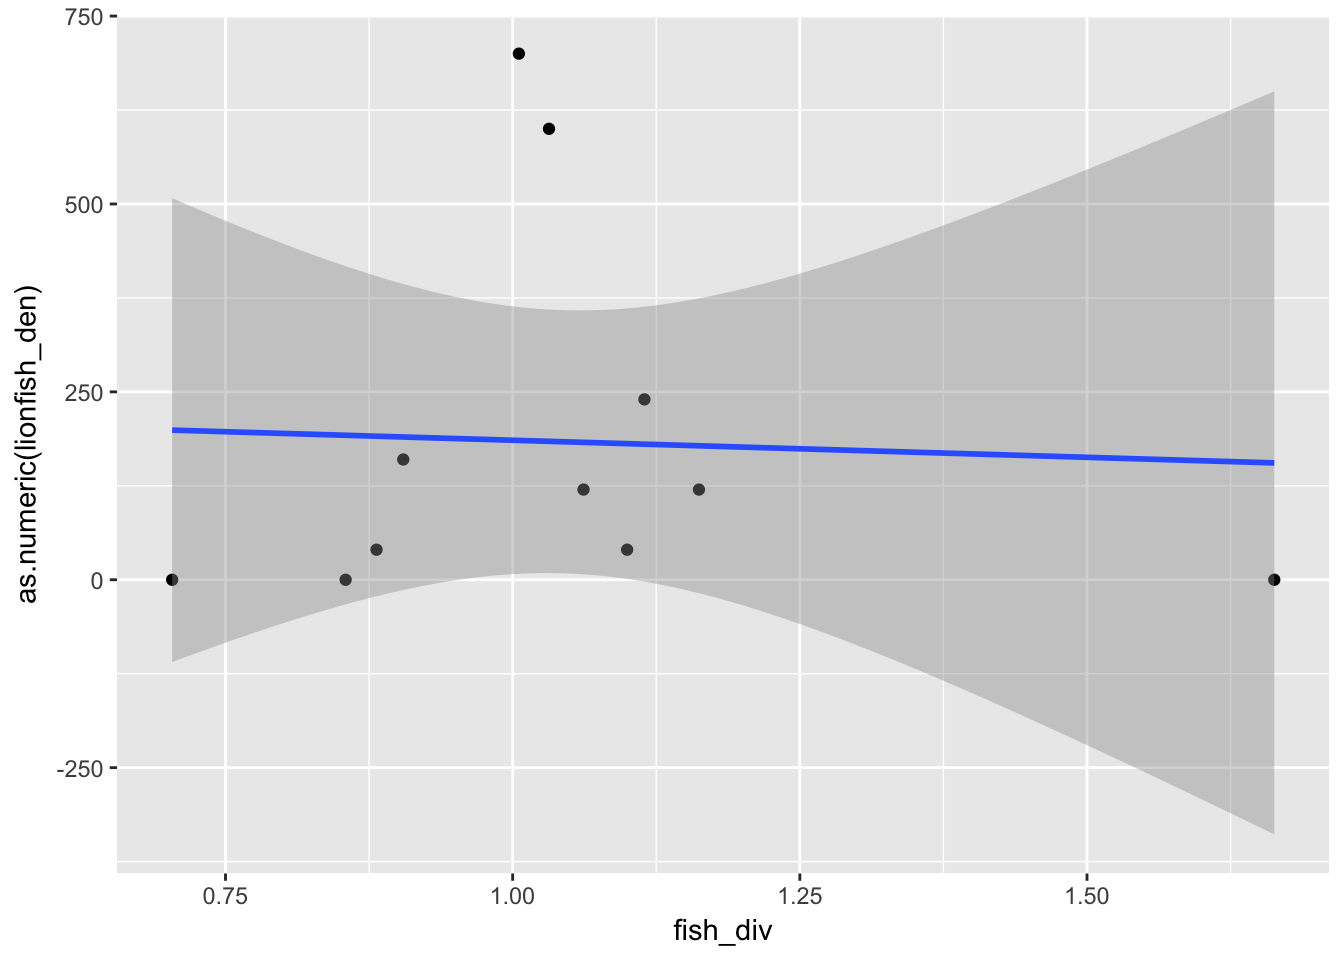
\includegraphics{heapmap_final_files/figure-latex/unnamed-chunk-3-1.pdf}
Changing color schemes

\begin{Shaded}
\begin{Highlighting}[]
\KeywordTok{ggplot}\NormalTok{(}\DataTypeTok{data =}\NormalTok{ heatmap, }\KeywordTok{aes}\NormalTok{(}\DataTypeTok{x =}\NormalTok{ site, }\DataTypeTok{y =}\NormalTok{ species)) }\OperatorTok{+}\StringTok{ }\KeywordTok{geom_tile}\NormalTok{(}\KeywordTok{aes}\NormalTok{(}\DataTypeTok{fill =}\NormalTok{ mean), }\DataTypeTok{color =} \StringTok{"white"}\NormalTok{) }\OperatorTok{+}
\StringTok{  }\KeywordTok{scale_fill_gradient}\NormalTok{(}\DataTypeTok{low =} \StringTok{"white"}\NormalTok{, }\DataTypeTok{high =} \StringTok{"darkred"}\NormalTok{) }\OperatorTok{+}
\StringTok{  }\KeywordTok{ylab}\NormalTok{(}\StringTok{"Species"}\NormalTok{) }\OperatorTok{+}
\StringTok{  }\KeywordTok{xlab}\NormalTok{(}\StringTok{""}\NormalTok{) }\OperatorTok{+}\StringTok{  }
\StringTok{  }\KeywordTok{theme}\NormalTok{(}\DataTypeTok{legend.title =} \KeywordTok{element_text}\NormalTok{(}\DataTypeTok{size =} \DecValTok{10}\NormalTok{),}
        \DataTypeTok{legend.text =} \KeywordTok{element_text}\NormalTok{(}\DataTypeTok{size =} \DecValTok{12}\NormalTok{),}
        \DataTypeTok{plot.title =} \KeywordTok{element_text}\NormalTok{(}\DataTypeTok{size=}\DecValTok{16}\NormalTok{),}
        \DataTypeTok{axis.title=}\KeywordTok{element_text}\NormalTok{(}\DataTypeTok{size=}\DecValTok{14}\NormalTok{,}\DataTypeTok{face=}\StringTok{"bold"}\NormalTok{),}
        \DataTypeTok{axis.text.x =} \KeywordTok{element_text}\NormalTok{(}\DataTypeTok{angle =} \DecValTok{45}\NormalTok{, }\DataTypeTok{hjust =} \DecValTok{1}\NormalTok{)) }\OperatorTok{+}
\StringTok{  }\KeywordTok{labs}\NormalTok{(}\DataTypeTok{fill =} \StringTok{"Percent"}\NormalTok{)}
\end{Highlighting}
\end{Shaded}

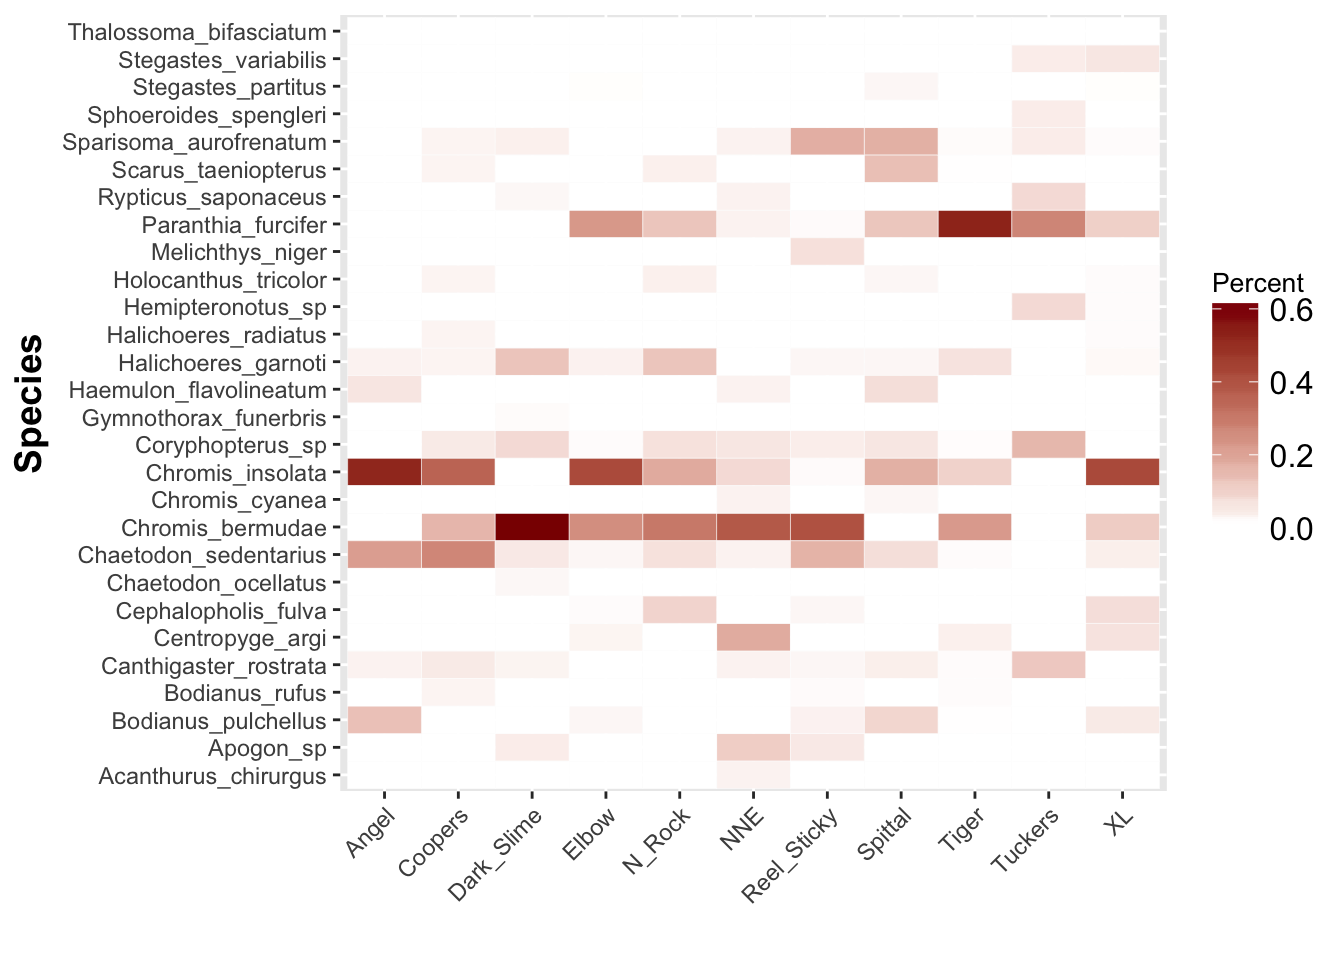
\includegraphics{heapmap_final_files/figure-latex/unnamed-chunk-4-1.pdf}
Changing the order of the fish species

\begin{Shaded}
\begin{Highlighting}[]
\KeywordTok{ggplot}\NormalTok{(}\DataTypeTok{data =}\NormalTok{ heatmap, }\KeywordTok{aes}\NormalTok{(}\DataTypeTok{x =}\NormalTok{ site, }\DataTypeTok{y =}\NormalTok{ species)) }\OperatorTok{+}\StringTok{ }\KeywordTok{geom_tile}\NormalTok{(}\KeywordTok{aes}\NormalTok{(}\DataTypeTok{y =} \KeywordTok{reorder}\NormalTok{(species, mean, median, }\DataTypeTok{order =} \OtherTok{TRUE}\NormalTok{), }\DataTypeTok{fill =}\NormalTok{ mean), }\DataTypeTok{color =} \StringTok{"white"}\NormalTok{) }\OperatorTok{+}
\StringTok{  }\KeywordTok{scale_fill_gradient}\NormalTok{(}\DataTypeTok{low =} \StringTok{"white"}\NormalTok{, }\DataTypeTok{high =} \StringTok{"darkblue"}\NormalTok{) }\OperatorTok{+}
\StringTok{  }\KeywordTok{ylab}\NormalTok{ (}\StringTok{"Species"}\NormalTok{) }\OperatorTok{+}
\StringTok{  }\KeywordTok{xlab}\NormalTok{(}\StringTok{""}\NormalTok{) }\OperatorTok{+}\StringTok{  }
\StringTok{  }\KeywordTok{theme}\NormalTok{(}\DataTypeTok{legend.title =} \KeywordTok{element_text}\NormalTok{(}\DataTypeTok{size =} \DecValTok{10}\NormalTok{),}
        \DataTypeTok{legend.text =} \KeywordTok{element_text}\NormalTok{(}\DataTypeTok{size =} \DecValTok{12}\NormalTok{),}
        \DataTypeTok{plot.title =} \KeywordTok{element_text}\NormalTok{(}\DataTypeTok{size=}\DecValTok{16}\NormalTok{),}
        \DataTypeTok{axis.title=}\KeywordTok{element_text}\NormalTok{(}\DataTypeTok{size=}\DecValTok{14}\NormalTok{,}\DataTypeTok{face=}\StringTok{"bold"}\NormalTok{),}
        \DataTypeTok{axis.text.x =} \KeywordTok{element_text}\NormalTok{(}\DataTypeTok{angle =} \DecValTok{45}\NormalTok{, }\DataTypeTok{hjust =} \DecValTok{1}\NormalTok{),}
\DataTypeTok{axis.text.y=}\KeywordTok{element_text}\NormalTok{(}\DataTypeTok{face=}\StringTok{"italic"}\NormalTok{)) }\OperatorTok{+}
\StringTok{  }\KeywordTok{labs}\NormalTok{(}\DataTypeTok{fill =} \StringTok{"Percent"}\NormalTok{)}
\end{Highlighting}
\end{Shaded}

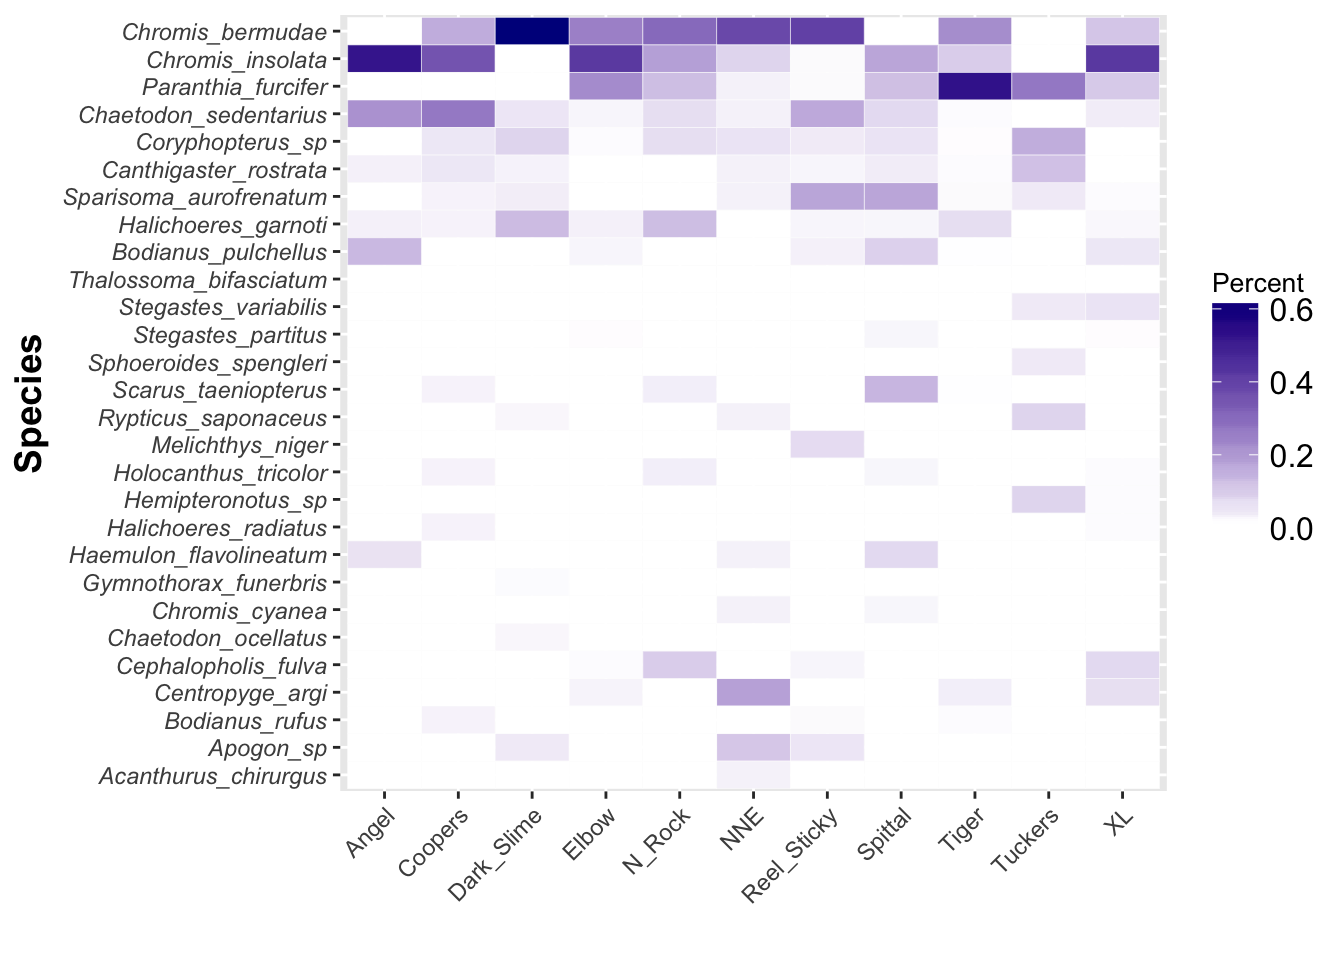
\includegraphics{heapmap_final_files/figure-latex/unnamed-chunk-5-1.pdf}

First version sent to review

\begin{Shaded}
\begin{Highlighting}[]
\NormalTok{heatmap_plot_red <-}\StringTok{ }\KeywordTok{ggplot}\NormalTok{(}\DataTypeTok{data =}\NormalTok{ heatmap, }\KeywordTok{aes}\NormalTok{(}\DataTypeTok{x =}\NormalTok{ site, }\DataTypeTok{y =}\NormalTok{ species)) }\OperatorTok{+}\StringTok{ }\KeywordTok{geom_tile}\NormalTok{(}\KeywordTok{aes}\NormalTok{(}\DataTypeTok{y =} \KeywordTok{reorder}\NormalTok{(species, mean, }\DataTypeTok{order =} \OtherTok{TRUE}\NormalTok{), }\DataTypeTok{fill =}\NormalTok{ mean), }\DataTypeTok{color =} \StringTok{"white"}\NormalTok{) }\OperatorTok{+}
\StringTok{  }\KeywordTok{scale_fill_gradient}\NormalTok{(}\DataTypeTok{low =} \StringTok{"white"}\NormalTok{, }\DataTypeTok{high =} \StringTok{"red"}\NormalTok{) }\OperatorTok{+}
\StringTok{  }\KeywordTok{ylab}\NormalTok{ (}\StringTok{"Species"}\NormalTok{) }\OperatorTok{+}
\StringTok{  }\KeywordTok{xlab}\NormalTok{(}\StringTok{""}\NormalTok{) }\OperatorTok{+}\StringTok{  }
\StringTok{  }\KeywordTok{theme}\NormalTok{(}\DataTypeTok{legend.title =} \KeywordTok{element_text}\NormalTok{(}\DataTypeTok{size =} \DecValTok{10}\NormalTok{),}
        \DataTypeTok{legend.text =} \KeywordTok{element_text}\NormalTok{(}\DataTypeTok{size =} \DecValTok{12}\NormalTok{),}
        \DataTypeTok{plot.title =} \KeywordTok{element_text}\NormalTok{(}\DataTypeTok{size=}\DecValTok{16}\NormalTok{),}
        \DataTypeTok{axis.title=}\KeywordTok{element_text}\NormalTok{(}\DataTypeTok{size=}\DecValTok{14}\NormalTok{,}\DataTypeTok{face=}\StringTok{"bold"}\NormalTok{),}
        \DataTypeTok{axis.text.x =} \KeywordTok{element_text}\NormalTok{(}\DataTypeTok{angle =} \DecValTok{45}\NormalTok{, }\DataTypeTok{hjust =} \DecValTok{1}\NormalTok{),}
\DataTypeTok{axis.text.y=}\KeywordTok{element_text}\NormalTok{(}\DataTypeTok{face=}\StringTok{"italic"}\NormalTok{)) }\OperatorTok{+}
\StringTok{  }\KeywordTok{labs}\NormalTok{(}\DataTypeTok{fill =} \StringTok{"Percent"}\NormalTok{)}
\NormalTok{heatmap_plot_red}
\end{Highlighting}
\end{Shaded}

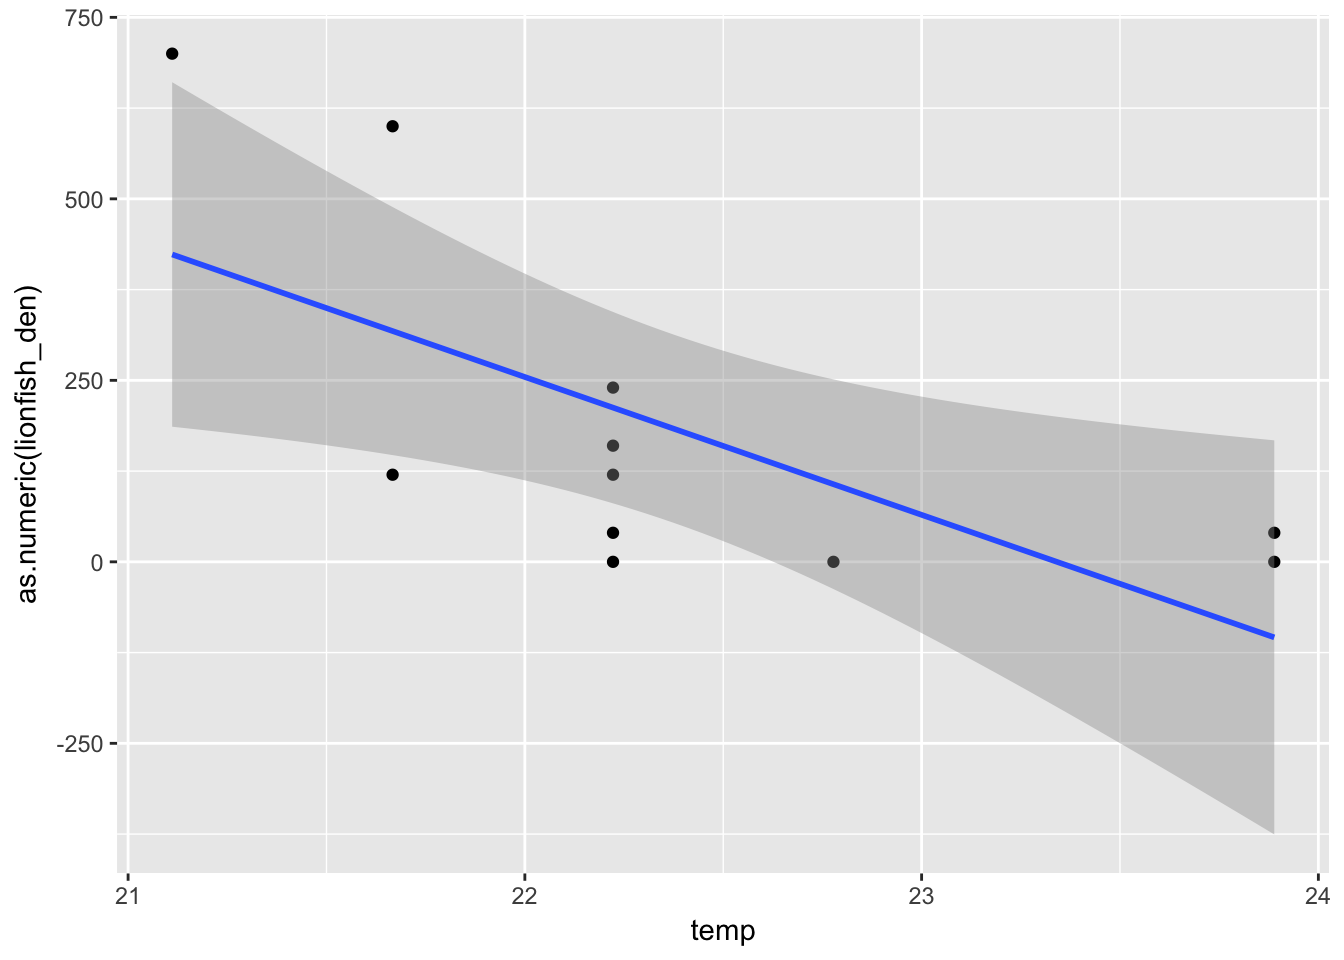
\includegraphics{heapmap_final_files/figure-latex/unnamed-chunk-6-1.pdf}

\begin{Shaded}
\begin{Highlighting}[]
\KeywordTok{ggsave}\NormalTok{(}\DataTypeTok{plot =}\NormalTok{ heatmap_plot_red, }\DataTypeTok{path=} \StringTok{"~/Desktop/Lionfish"}\NormalTok{, }\DataTypeTok{filename =} \StringTok{"heatmap_plot_red_rev.eps"}\NormalTok{, }\DataTypeTok{device =} \StringTok{"eps"}\NormalTok{)}
\end{Highlighting}
\end{Shaded}

\begin{verbatim}
## Saving 6.5 x 4.5 in image
\end{verbatim}

Modifications made based on reviewer comments, including changing the
x-axis to reorder sites in clockwise location around Bermuda and using
mean instead of median for the order of the species.

\begin{Shaded}
\begin{Highlighting}[]
\CommentTok{# reorder x axis to go around the platform}
\CommentTok{# mtcars$cyl2 <- factor(mtcars$cyl, levels = c("6","4","8"))}
\NormalTok{heatmap}\OperatorTok{$}\NormalTok{site <-}\StringTok{ }\KeywordTok{as.character}\NormalTok{(heatmap}\OperatorTok{$}\NormalTok{site)}
\NormalTok{heatmap}\OperatorTok{$}\NormalTok{site <-}\StringTok{ }\KeywordTok{factor}\NormalTok{(heatmap}\OperatorTok{$}\NormalTok{site, }\DataTypeTok{levels =} \KeywordTok{c}\NormalTok{(}\StringTok{"Angel"}\NormalTok{, }\StringTok{"Dark_Slime"}\NormalTok{, }\StringTok{"N_Rock"}\NormalTok{, }\StringTok{"Reel_Sticky"}\NormalTok{, }\StringTok{"NNE"}\NormalTok{, }\StringTok{"XL"}\NormalTok{, }\StringTok{"Coopers"}\NormalTok{, }\StringTok{"Tuckers"}\NormalTok{, }\StringTok{"Spittal"}\NormalTok{, }\StringTok{"Elbow"}\NormalTok{, }\StringTok{"Tiger"}\NormalTok{))}
\NormalTok{heatmap_plot_rev <-}\StringTok{ }\KeywordTok{ggplot}\NormalTok{(}\DataTypeTok{data =}\NormalTok{ heatmap, }\KeywordTok{aes}\NormalTok{(}\DataTypeTok{x =}\NormalTok{ site, }\DataTypeTok{y =}\NormalTok{ species)) }\OperatorTok{+}\StringTok{ }\KeywordTok{geom_tile}\NormalTok{(}\KeywordTok{aes}\NormalTok{(}\DataTypeTok{y =} \KeywordTok{reorder}\NormalTok{(species, mean, }\DataTypeTok{order =} \OtherTok{TRUE}\NormalTok{), }\DataTypeTok{fill =}\NormalTok{ mean), }\DataTypeTok{color =} \StringTok{"white"}\NormalTok{) }\OperatorTok{+}
\StringTok{  }\KeywordTok{scale_fill_gradient}\NormalTok{(}\DataTypeTok{low =} \StringTok{"white"}\NormalTok{, }\DataTypeTok{high =} \StringTok{"red"}\NormalTok{) }\OperatorTok{+}
\StringTok{  }\KeywordTok{ylab}\NormalTok{ (}\StringTok{"Species"}\NormalTok{) }\OperatorTok{+}
\StringTok{  }\KeywordTok{xlab}\NormalTok{(}\StringTok{""}\NormalTok{) }\OperatorTok{+}\StringTok{ }\KeywordTok{theme_classic}\NormalTok{() }\OperatorTok{+}
\StringTok{  }\KeywordTok{theme}\NormalTok{(}\DataTypeTok{legend.title =} \KeywordTok{element_text}\NormalTok{(}\DataTypeTok{size =} \DecValTok{10}\NormalTok{),}
        \DataTypeTok{legend.text =} \KeywordTok{element_text}\NormalTok{(}\DataTypeTok{size =} \DecValTok{12}\NormalTok{),}
        \DataTypeTok{plot.title =} \KeywordTok{element_text}\NormalTok{(}\DataTypeTok{size=}\DecValTok{16}\NormalTok{),}
        \DataTypeTok{axis.title=}\KeywordTok{element_text}\NormalTok{(}\DataTypeTok{size=}\DecValTok{14}\NormalTok{,}\DataTypeTok{face=}\StringTok{"bold"}\NormalTok{),}
        \DataTypeTok{axis.text.x =} \KeywordTok{element_text}\NormalTok{(}\DataTypeTok{angle =} \DecValTok{45}\NormalTok{, }\DataTypeTok{hjust =} \DecValTok{1}\NormalTok{),}
\DataTypeTok{axis.text.y=}\KeywordTok{element_text}\NormalTok{(}\DataTypeTok{face=}\StringTok{"italic"}\NormalTok{)) }\OperatorTok{+}
\StringTok{  }\KeywordTok{labs}\NormalTok{(}\DataTypeTok{fill =} \StringTok{"Percent"}\NormalTok{)}
\NormalTok{heatmap_plot_rev}
\end{Highlighting}
\end{Shaded}

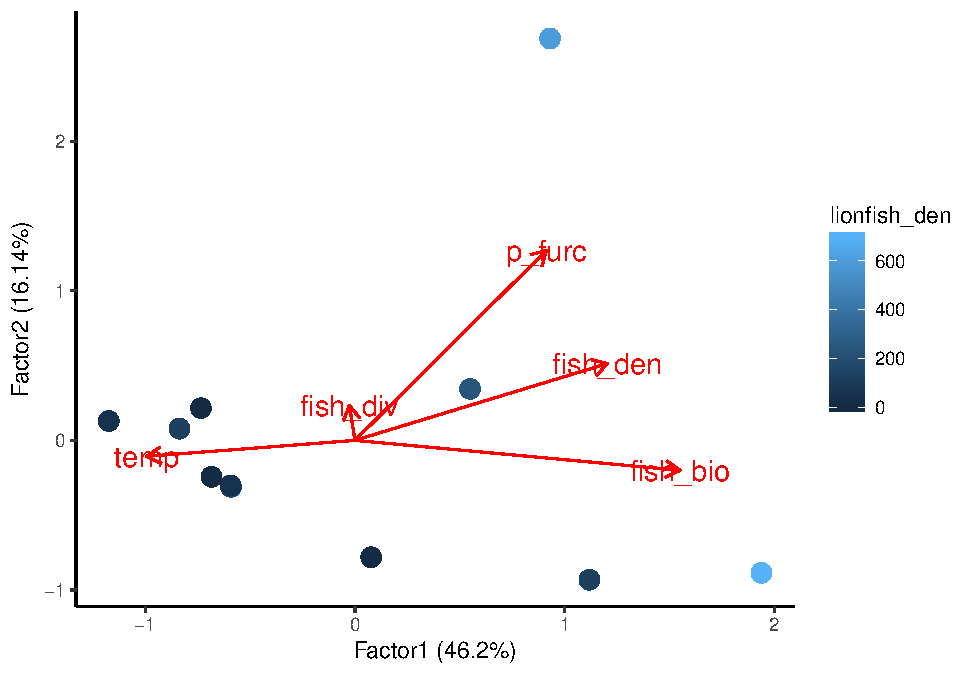
\includegraphics{heapmap_final_files/figure-latex/unnamed-chunk-7-1.pdf}

\begin{Shaded}
\begin{Highlighting}[]
\KeywordTok{ggsave}\NormalTok{(}\DataTypeTok{plot =}\NormalTok{ heatmap_plot_rev, }\DataTypeTok{path=} \StringTok{"~/Desktop/Lionfish"}\NormalTok{, }\DataTypeTok{filename =} \StringTok{"heatmap_plot_rev.eps"}\NormalTok{, }\DataTypeTok{device =} \StringTok{"eps"}\NormalTok{)}
\end{Highlighting}
\end{Shaded}

\begin{verbatim}
## Saving 6.5 x 4.5 in image
\end{verbatim}

Adjusting colors and font size

\begin{Shaded}
\begin{Highlighting}[]
\NormalTok{heatmap}\OperatorTok{$}\NormalTok{site <-}\StringTok{ }\KeywordTok{as.character}\NormalTok{(heatmap}\OperatorTok{$}\NormalTok{site)}
\NormalTok{heatmap}\OperatorTok{$}\NormalTok{site <-}\StringTok{ }\KeywordTok{factor}\NormalTok{(heatmap}\OperatorTok{$}\NormalTok{site, }\DataTypeTok{levels =} \KeywordTok{c}\NormalTok{(}\StringTok{"Angel"}\NormalTok{, }\StringTok{"Dark_Slime"}\NormalTok{, }\StringTok{"N_Rock"}\NormalTok{, }\StringTok{"Reel_Sticky"}\NormalTok{, }\StringTok{"NNE"}\NormalTok{, }\StringTok{"XL"}\NormalTok{, }\StringTok{"Coopers"}\NormalTok{, }\StringTok{"Tuckers"}\NormalTok{, }\StringTok{"Spittal"}\NormalTok{, }\StringTok{"Elbow"}\NormalTok{, }\StringTok{"Tiger"}\NormalTok{))}
\NormalTok{heatmap_plot_revBP <-}\StringTok{ }\KeywordTok{ggplot}\NormalTok{(}\DataTypeTok{data =}\NormalTok{ heatmap, }\KeywordTok{aes}\NormalTok{(}\DataTypeTok{x =}\NormalTok{ site, }\DataTypeTok{y =}\NormalTok{ species)) }\OperatorTok{+}\StringTok{ }\KeywordTok{geom_tile}\NormalTok{(}\KeywordTok{aes}\NormalTok{(}\DataTypeTok{y =} \KeywordTok{reorder}\NormalTok{(species, mean, }\DataTypeTok{order =} \OtherTok{TRUE}\NormalTok{), }\DataTypeTok{fill =}\NormalTok{ mean), }\DataTypeTok{color =} \StringTok{"white"}\NormalTok{) }\OperatorTok{+}
\StringTok{  }\KeywordTok{scale_fill_gradient2}\NormalTok{(}\DataTypeTok{low =} \StringTok{"white"}\NormalTok{, }\DataTypeTok{high =} \StringTok{"darkred"}\NormalTok{, }\DataTypeTok{mid =} \StringTok{"red"}\NormalTok{, }\DataTypeTok{midpoint =} \FloatTok{0.31}\NormalTok{) }\OperatorTok{+}
\StringTok{  }\KeywordTok{ylab}\NormalTok{ (}\StringTok{"Species"}\NormalTok{) }\OperatorTok{+}
\StringTok{  }\KeywordTok{xlab}\NormalTok{(}\StringTok{""}\NormalTok{) }\OperatorTok{+}\StringTok{ }\KeywordTok{theme_classic}\NormalTok{() }\OperatorTok{+}
\StringTok{  }\KeywordTok{theme}\NormalTok{(}\DataTypeTok{legend.title =} \KeywordTok{element_text}\NormalTok{(}\DataTypeTok{size =} \DecValTok{10}\NormalTok{),}
        \DataTypeTok{legend.text =} \KeywordTok{element_text}\NormalTok{(}\DataTypeTok{size =} \DecValTok{12}\NormalTok{),}
        \DataTypeTok{plot.title =} \KeywordTok{element_text}\NormalTok{(}\DataTypeTok{size=}\DecValTok{16}\NormalTok{),}
        \DataTypeTok{axis.title=}\KeywordTok{element_text}\NormalTok{(}\DataTypeTok{size=}\DecValTok{14}\NormalTok{),}
        \DataTypeTok{axis.text.x =} \KeywordTok{element_text}\NormalTok{(}\DataTypeTok{angle =} \DecValTok{45}\NormalTok{, }\DataTypeTok{hjust =} \DecValTok{1}\NormalTok{, }\DataTypeTok{size =} \DecValTok{12}\NormalTok{),}
\DataTypeTok{axis.text.y=}\KeywordTok{element_text}\NormalTok{(}\DataTypeTok{face=}\StringTok{"italic"}\NormalTok{, }\DataTypeTok{size =} \DecValTok{12}\NormalTok{)) }\OperatorTok{+}
\StringTok{  }\KeywordTok{labs}\NormalTok{(}\DataTypeTok{fill =} \StringTok{"Percent Contribution"}\NormalTok{)}
\NormalTok{heatmap_plot_revBP}
\end{Highlighting}
\end{Shaded}

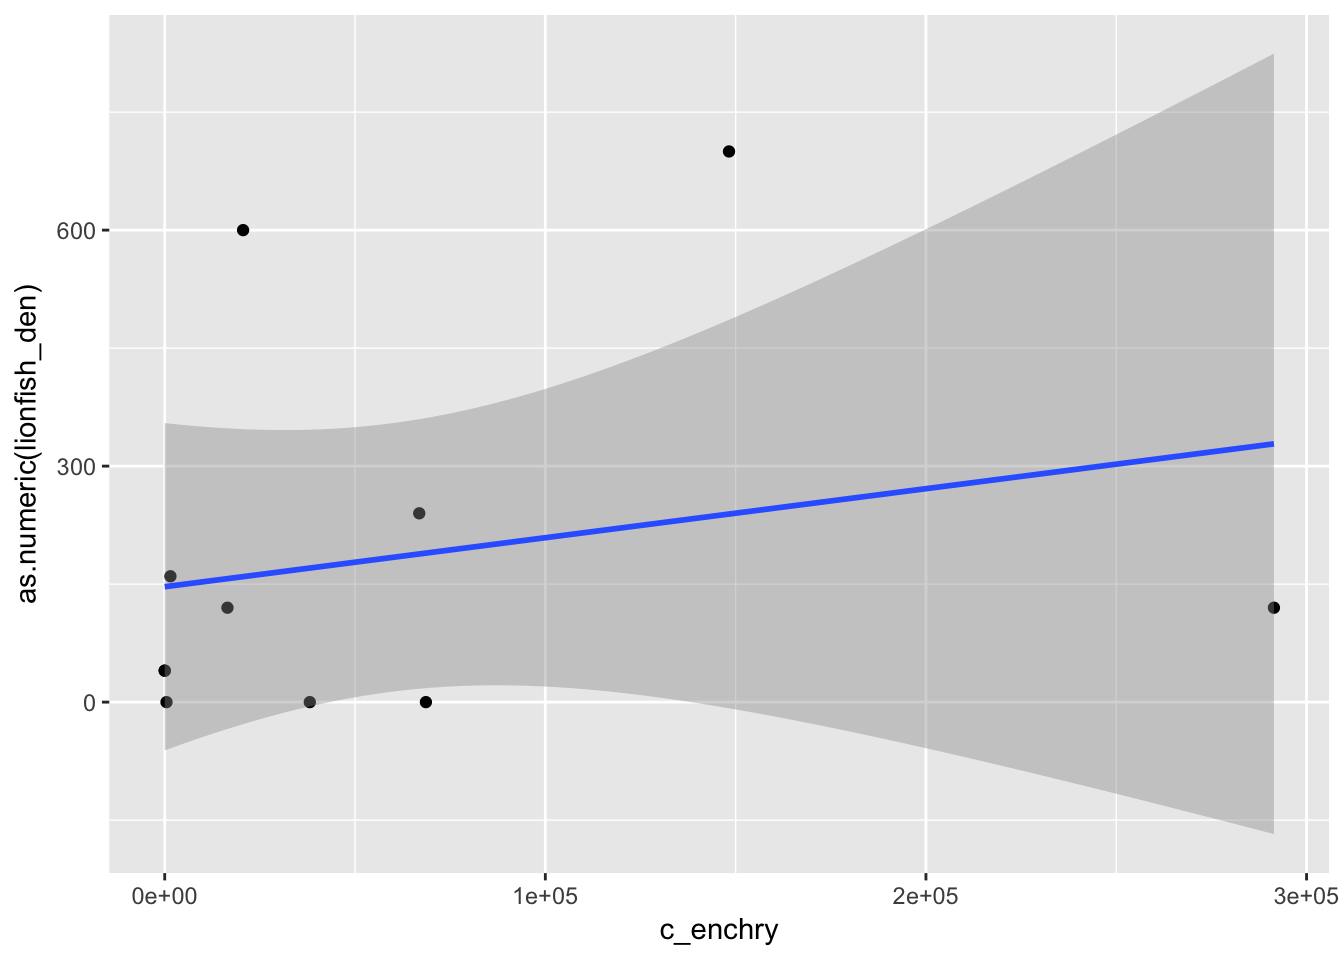
\includegraphics{heapmap_final_files/figure-latex/unnamed-chunk-8-1.pdf}

\begin{Shaded}
\begin{Highlighting}[]
\KeywordTok{ggsave}\NormalTok{(}\DataTypeTok{plot =}\NormalTok{ heatmap_plot_revBP, }\DataTypeTok{path=} \StringTok{"~/Desktop/Lionfish"}\NormalTok{, }\DataTypeTok{filename =} \StringTok{"heatmap_final.eps"}\NormalTok{, }\DataTypeTok{device =} \StringTok{"eps"}\NormalTok{)}
\end{Highlighting}
\end{Shaded}

\begin{verbatim}
## Saving 6.5 x 4.5 in image
\end{verbatim}

Final Version in publication

\begin{Shaded}
\begin{Highlighting}[]
\NormalTok{heatmap}\OperatorTok{$}\NormalTok{site <-}\StringTok{ }\KeywordTok{as.character}\NormalTok{(heatmap}\OperatorTok{$}\NormalTok{site)}
\NormalTok{heatmap}\OperatorTok{$}\NormalTok{site <-}\StringTok{ }\KeywordTok{factor}\NormalTok{(heatmap}\OperatorTok{$}\NormalTok{site, }\DataTypeTok{levels =} \KeywordTok{c}\NormalTok{(}\StringTok{"Angel"}\NormalTok{, }\StringTok{"Dark_Slime"}\NormalTok{, }\StringTok{"N_Rock"}\NormalTok{, }\StringTok{"Reel_Sticky"}\NormalTok{, }\StringTok{"NNE"}\NormalTok{, }\StringTok{"XL"}\NormalTok{, }\StringTok{"Coopers"}\NormalTok{, }\StringTok{"Tuckers"}\NormalTok{, }\StringTok{"Spittal"}\NormalTok{, }\StringTok{"Elbow"}\NormalTok{, }\StringTok{"Tiger"}\NormalTok{))}
\NormalTok{heatmap_plot_revBP <-}\StringTok{ }\KeywordTok{ggplot}\NormalTok{(}\DataTypeTok{data =}\NormalTok{ heatmap, }\KeywordTok{aes}\NormalTok{(}\DataTypeTok{x =}\NormalTok{ site, }\DataTypeTok{y =}\NormalTok{ species)) }\OperatorTok{+}\StringTok{ }\KeywordTok{geom_tile}\NormalTok{(}\KeywordTok{aes}\NormalTok{(}\DataTypeTok{y =} \KeywordTok{reorder}\NormalTok{(species, mean, }\DataTypeTok{order =} \OtherTok{TRUE}\NormalTok{), }\DataTypeTok{fill =}\NormalTok{ mean), }\DataTypeTok{color =} \StringTok{"white"}\NormalTok{) }\OperatorTok{+}
\StringTok{  }\KeywordTok{scale_fill_gradient2}\NormalTok{(}\DataTypeTok{low =} \StringTok{"white"}\NormalTok{, }\DataTypeTok{high =} \StringTok{"darkred"}\NormalTok{, }\DataTypeTok{mid =} \StringTok{"red"}\NormalTok{, }\DataTypeTok{midpoint =} \FloatTok{0.31}\NormalTok{) }\OperatorTok{+}
\StringTok{  }\KeywordTok{ylab}\NormalTok{ (}\StringTok{"Species"}\NormalTok{) }\OperatorTok{+}
\StringTok{  }\KeywordTok{xlab}\NormalTok{(}\StringTok{""}\NormalTok{) }\OperatorTok{+}\StringTok{ }\KeywordTok{theme_bw}\NormalTok{() }\OperatorTok{+}
\StringTok{  }\KeywordTok{theme}\NormalTok{(}\DataTypeTok{legend.title =} \KeywordTok{element_text}\NormalTok{(}\DataTypeTok{size =} \DecValTok{10}\NormalTok{),}
        \DataTypeTok{legend.text =} \KeywordTok{element_text}\NormalTok{(}\DataTypeTok{size =} \DecValTok{12}\NormalTok{),}
        \DataTypeTok{plot.title =} \KeywordTok{element_text}\NormalTok{(}\DataTypeTok{size=}\DecValTok{16}\NormalTok{),}
        \DataTypeTok{axis.title=}\KeywordTok{element_text}\NormalTok{(}\DataTypeTok{size=}\DecValTok{14}\NormalTok{),}
        \DataTypeTok{axis.text.x =} \KeywordTok{element_text}\NormalTok{(}\DataTypeTok{angle =} \DecValTok{45}\NormalTok{, }\DataTypeTok{hjust =} \DecValTok{1}\NormalTok{),}
\DataTypeTok{axis.text.y=}\KeywordTok{element_text}\NormalTok{(}\DataTypeTok{face=}\StringTok{"italic"}\NormalTok{)) }\OperatorTok{+}
\StringTok{  }\KeywordTok{labs}\NormalTok{(}\DataTypeTok{fill =} \StringTok{"Percent Contribution"}\NormalTok{)}
\NormalTok{heatmap_plot_revBP}
\end{Highlighting}
\end{Shaded}

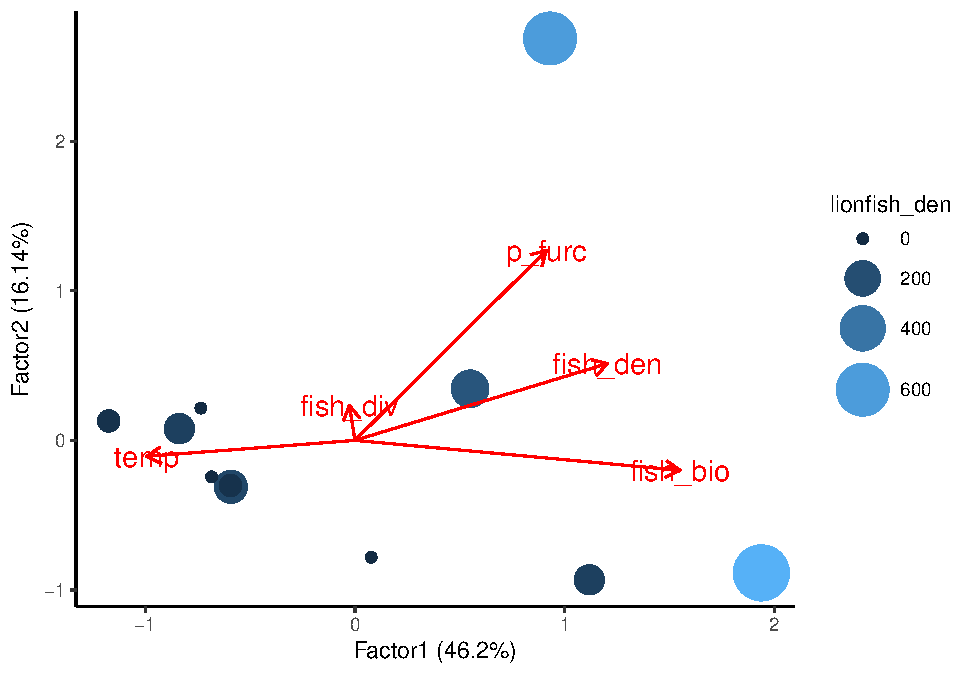
\includegraphics{heapmap_final_files/figure-latex/unnamed-chunk-9-1.pdf}

\begin{Shaded}
\begin{Highlighting}[]
\KeywordTok{ggsave}\NormalTok{(}\DataTypeTok{plot =}\NormalTok{ heatmap_plot_revBP, }\DataTypeTok{path=} \StringTok{"~/Desktop/Lionfish"}\NormalTok{, }\DataTypeTok{filename =} \StringTok{"heatmap_final2.eps"}\NormalTok{, }\DataTypeTok{device =} \StringTok{"eps"}\NormalTok{)}
\end{Highlighting}
\end{Shaded}

\begin{verbatim}
## Saving 6.5 x 4.5 in image
\end{verbatim}


\end{document}
